\section{Approach}\label{sec:approach}

In this paper, we propose a tool to create custom memory profilers for managed runtime environments (MREs) such as Java.
We are interested on easing the task of defining new profilers without sacrificing their performance regarding CPU consumption.
Keeping the profiler's overhead as low as possible is of utmost importance for us because lightweight profilers can be use both during the development phase and during the application execution in a production environment.
To reach this goal, we propose a Domain Specific Language (DSL) and its code generator which aims at describing and generating efficient online memory profilers. 

We next present the syntax, semantic and usage examples of our domain-specific language.


\subsection{Brief overview of the domain}

Memory profilers aim at capturing information regarding how an application use memory.
In an object-oriented runtime environment such as Java, this information can be as simple as the number of objects of a specific class, but it can also be  as complex  as the list of possible memory leak sources.
Along this paper, the term memory profiler refers to any kind of process to retrieve data about the memory usage.
Some examples include: computing the number of objects reachable from a specific class object; finding out if there is an instance of class $A$ which is referencing an instance of class $B$.
A last example could be computing for each instance of the class \textit{String} its length and the number of references to it.
It is worth mentioning that the data collected by a profiler may have an arbitrary type.
For instance, in the previous examples the types are primitives integer, boolean and a non-primitive type.

%The rest of this section introduces the vocabulary we use in the domain of memory profilers.

In this paper, we are interested in \textbf{\textit{objects}} as in object-oriented programming.
We also see an \textit{object} as an atomic entity that consumes memory to store the values of its attributes.
We have  reduced the available operations on objects to: accessing attributes, obtaining the amount of memory used to represent the object, and accessing meta-data such as the class name.

The \textbf{\textit{memory heap}} is the region of memory used to store dynamically allocated \textit{objects}.
Although this concept is pervasive in general purposes programming languages, we are only interested on MREs such as Java where every \textit{object} must be allocated in this region.

A \textbf{\textit{structure}} is an important concept in our domain.
It consists of a set of related \textit{objects} in the \textit{memory heap}.
The smallest non-empty \textit{structure} we can consider, is a structure containing a single object.
The \textit{memory heap} is the universe of objects and each \textit{structure} is a subset of this universe.

A \textbf{\textit{memory profile}} is a value associated to a \textit{structure} which can be derived out of the indivdual \textit{objects} included in the \textit{structure}. 
An example of useful derived value for a \textit{structure} is its total size: $\textit{total\_size(S)} = \sum_{o \in S} {sizeof(o)}$.
A common usage is to identify many \textit{structures} in the heap to obtain a \textit{memory profile} for each of them.
These two steps: identifying \textit{structures} and computing their \textit{memory profile} correspond to what we call \textbf{\textit{memory profiling}}. 

Finally, a \textbf{\textit{structure type}} provides a description of the behavior of a set of \textit{structures}. 
In particular, it provides (i) a function to evaluate whether an object is member of the \textit{structure}, (ii) a way to define the values corresponding to the \textit{memory profile} of the \textit{structure}, and finally (iii) a factory to identify all  corresponding \textit{structures} in the \textit{memory heap}.

\subsection{Abstract Syntax}\label{sec:abstract-syntax}

The metamodel shown in figure~\ref{fig:as} describes the abstract syntax of our DSL.
The main concept of this metamodel is a \textit{CustomProfiler} which is composed of \textit{UserDefined} types and a \textit{StructureFactory}.
The concepts related to \textit{UserDefined} types are shown on the left part of the metamodel, while the right part describes the \textit{StructureFactory} which represents both the set of  structures to identify and the value to compute on these structures.

\subsubsection{User-defined types}
In addition to various \textit{BasicTypes} such as \textit{Integer}, \textit{String} and \textit{Boolean}, the language supports the definition of both \textit{Records} and \textit{Lists}.
As expected, a \textit{record} contains \textit{fields} to hold values of previously defined types.
Likewise, a \textit{list} refer to a \textit{base type}; hence all the members of a list must be of the same type.
In a custom profiler, \textit{UserDefined} types can be composed in arbitrary ways as long as no type contains a recursive declaration.
We can formalize such a constrain using OCL (Object Constraint Language~\footnote{http://www.omg.org/spec/OCL/}):

\begin{lstlisting}[escapeinside={(*}{*)}, label=fig:membership, language=OCL, frame=none, aboveskip=2mm, belowskip=2mm]
context Record inv: 
   not fields->oclAsSet()->closure(t)->exists(t | t = self)

context List inv:
   not baseType->oclAsSet()->closure(t)->exists(t | t = self)
\end{lstlisting} 

A \textit{List} has operations to manipulate any value which represent a list.
Figure~\ref{fig:as} shows a subset of these operations.
In general, these operations correspond to the set of \textit{standard} operations of any implementation of the list data type.

\subsubsection{Defining structures to profile}
Defining the \textit{StructureFactory} is the core of writing a custom profiler.
A \textit{StructureFactory} contains an \textit{Expression} through the \textit{instances} relationship which indicates a pattern to identify structures in the memory heap.
Notice that a single instance of \textit{StructureFactory} creates many data structures in memory; thus the \textit{Expression} corresponds to a list indicating that a new structure must be instantiated for each element of the list.
Forcing the \textit{Expression} to be a \textit{List} can be easily formalized using OCL:

\begin{lstlisting}[escapeinside={(*}{*)}, label=fig:instances, language=OCL, frame=none, aboveskip=2mm, belowskip=2mm]
context StructureFactory inv: instances.type.oclIsTypeOf(List)
\end{lstlisting}

Defining a new \textit{StructureFactory} implies defining its \textit{type} which is an instance of \textit{StructureType}.
This concept describes the mechanism used to populate, out of objects, a structure and its information.
In short, each structure in memory instanciated through a \textit{StructureFactory} has a type \textit{StructureType}.
For example, we may be interested in finding all the \textit{SimplyLinkedList} in the memory snapshot depicted in figure~\ref{fig:simple_snapshot}.
In such a case, there are two \textit{SimplyLinkedList}, but we only need one mechanism to identify them because they have the same pattern in memory. 

\begin{figure*}
\centering
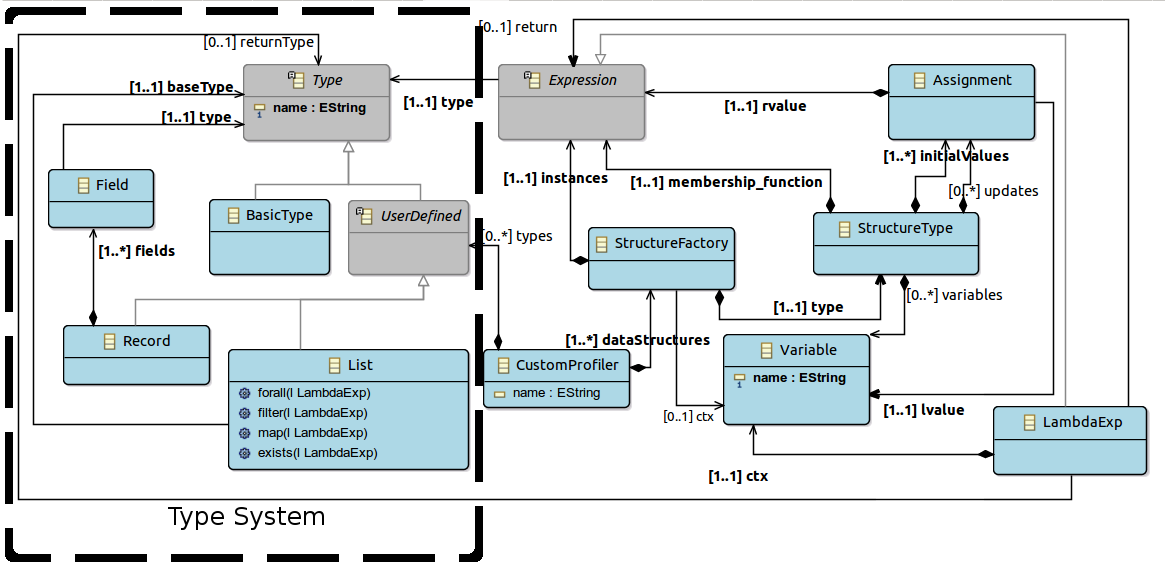
\includegraphics[width=0.87\linewidth]{chapter6/fig/AS}
\caption{Custom profiler Metamodel}
\label{fig:as}
\end{figure*}

\begin{figure}
\centering
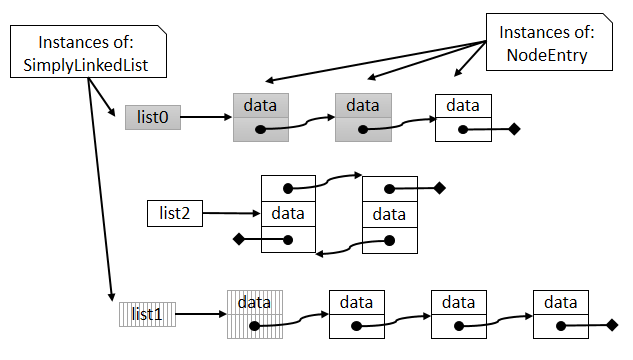
\includegraphics[width=0.87\linewidth]{chapter6/fig/lists}
\caption{Memory snapshot with three linked lists}
\label{fig:simple_snapshot}
\end{figure}

A \textit{StructureType} is composed of \textit{Assignments} that are used as \textit{initialValues} for each \textit{Variable} holding information - similar to a constructor in object-oriented programming.
Once a new structure is created, the \textit{Assignments} are executed to assign the initial value of each \textit{Variable}.
Observe that \textit{variables} do not refer to a \textit{Type}.
Our DSL is strongly typed and the \textit{type} of each user-defined variable is inferred from its initial value.
Nevertheless, there is a built-in variable in each \textit{StructureType} that is only accessible during initialization.
Its type is predetermined as part of the language specification.
We force the usage of the proper type using OCL:

\begin{lstlisting}[escapeinside={(*}{*)}, label=fig:instances, language=OCL, frame=none, aboveskip=2mm, belowskip=2mm]
context StructureType inv:  initialValues->exists(a: Assignment | 
     a.lvalue.name = 'initialObjects' and a.rvalue.type.oclIsTypeOf(List)
   ) 
\end{lstlisting}

In addition, a \textit{StructureType} contains a boolean \textit{expression} which is the \textit{membership function} used to decide whether an object should be included in the structure instance.
Finally, it also contains a set of \textit{Assignments} to update the value of each \textit{variable} every time a new object is included in the structure.
This set of \textit{Assignments} is used to compute the actual value of the memory profile.
The major constraint regarding these \textit{updates} is that they must refer to already initialized \textit{variables} and the new assigned values must match the previous types.
We formalize such a constrain using OCL:

\begin{lstlisting}[escapeinside={(*}{*)}, label=fig:lvalue, language=OCL, frame=none, aboveskip=2mm, belowskip=2mm]
context StructureType inv:  updates->forAll(a: Assignament | 
    self.initialValues->exists(aa : Assignament | 
       aa.lvalue = a.lvalue and aa.rvalue.type = a.rvalue.type
     ))
\end{lstlisting}

In our DSL, \textit{expressions} play a big role.
For the sake of readability, figure~\ref{fig:as} only shows a couple of concepts related to them.
However, it is noteworthy that, in addition to \textit{arithmetic}, \textit{boolean} and \textit{literals} for basic types, the language includes lambda expressions, literal for records and lists.
Moreover, the language defines \textit{built-in rvalues} which are nothing but expressions initialized by the runtime within a specific scope.
Instead of being user-defined, the types of these expressions are also defined by the runtime.
There are two types of \textit{built-in rvalues}, target independent and dependent.
Among the firsts, we have the list of  \textit{objects}, a reference to the \textit{current data structure} and a reference to the \textit{current object}.
Target dependent \textit{rvalues} in Java include the list of \textit{loaded classes} and the list of \textit{threads}.
The precise meaning of these \textit{rvalues} as well as their scopes are precisely discussed in sections~\ref{sec:concrete-syntax}, ~\ref{sec:semantic} and~\ref{sec:implementation} along the concrete syntax, the language semantic and the tooling support.

Finally, if we use the memory snapshot depicted in figure~\ref{fig:simple_snapshot}, calculating the number of nodes belonging to a specific \textit{SimplyLinkedList} is an example that illustrates the language's concepts.
To solve this problem we can instantiate the metamodel of our DSL as follow:
\begin{itemize}
\item Define a \textit{StructureFactory} in which the \textit{instances} property is a list which contains the objects \textit{list0} and \textit{list1}.
\item Instantiate a \textit{StructureType} where the built-in variable \textit{initialObjects} receives as value a list with one member - list0 or list1.
      The other properties of this \textit{StructureType} instance are detailed in the next steps: 
      \begin{enumerate}
      \item Define a variable \textit{n} with initial value zero.
      \item Define a membership function which return true if an object is instance of \textit{NodeEntry} and it is referenced by an object for which the membership function also return true. Observe how this recursive function returns true for each element in \textit{list0} because the initial object's list contains object \textit{list0}. 
      \item Update the variable \textit{n} by increasing its value by one.
      \end{enumerate}  
\end{itemize}
Further details about this example are discussed in the next section.

\subsection{Concrete Syntax}\label{sec:concrete-syntax}

A textual concrete syntax has been defined for our DSL allowing the domain expert to define a custom memory profiler.
As an example, the next listing shows how to compute the length of each \textit{SimplyLinkedList} in the memory snapshot depicted in figure~\ref{fig:simple_snapshot}.
The mechanism is based on counting the number of \textit{NodeEntry} referenced by the \textit{SimplyLinkedList}.
Each \textit{NodeEntry} is used to wrap one element of data and to point to the next element.

\begin{lstlisting}[escapeinside={(*}{*)}, 
label=lst:listLengt, language=DSL2,
numbersep=2pt,
numbers=left,
numberstyle=\color{black}\scriptsize,
frame=none
]
create structure foreach e:objects.filter(l| l is SimplyLinkedList) using
  constructor
    initialObjects = #[e] // a list literal with one element: e
    n = 0
  membership (this is NodeEntry) and (referrer in this_structure)
  updates 
    n = n + 1
\end{lstlisting}

In the example, only one \textit{StructureFactory} is necessary.
In line 1, we define the list of structures we are interested in.
We do so by selecting instances of class \textit{SimplyLinkedList} as elements of the \textit{StructureFactory}.
Since there are two simply linked lists in the memory snapshot, we are going to build two structures.
Observe the usage of a built-in \textit{rvalue} named \textit{objects} which contains all the objects in memory.
The valid scope of this rvalue is in both the definition of the set of structures and the computation of the initial values.
Thereafter, lines 2-4 specify the initial values.
Line 3 in particular initializes the set of objects included in the structure.
Notice the usage of a list literal to include the object referenced by \textit{e}.
In the initialization scope, the rvalue \textit{e} is equal to one of the element within the list of structures - either \textit{list0} or \textit{list1}.

In line 6 we define the membership function, which is used to determine if an object is part of the structure.
There are four built-in rvalues during the evaluation of the function as well as during the update of the variables.
First, the value named \textit{this} is the current visited object. 
The \textit{membership} boolean \textit{expression} aims at determining if this object is part of the \textit{structure} or not. 
The value \textit{this\_structure} identifies the structure.
As our runtime profiler will traverse the graph of in memory objects following references between objects, the object through which we have reached the \textit{this} object is known as \textit{referrer}.
The last value, which is target dependent, is the kind of reference.
Operator \textbf{is} checks if \textit{this} is an instance of class \textit{NodeEntry}.
Likewise, operator \textbf{in} checks whether the \textit{referrer} is already a member of the structure.
Finally, line 8 updates the length of the list when an object is detected as member of the structure.

\subsection{Semantics}\label{sec:semantic}

An instance of our metamodel is compiled into a custom memory profiler.
This compilation produces a library written in \textit{C++} which is in charge of collecting the desired information from the runtime environment.
The generated source code has two parts.
First, for each \textit{StructureType} in the model, the compiler generates a subclass of \textit{AbstractStructureType} which is shown below.
Every subclass contains attributes to store the variables used in the associated \textit{StructureType}.
In the listing below, the class \textit{Context} holds the built-in values we mention in the previous section.
\begin{lstlisting}[language=C++, frame=none,
numbers=left,
numberstyle=\color{black}\scriptsize,]
class AbstractStructureType {
public:
	void initialize(Context& ctx) = 0;
	bool membership(Context& ctx) = 0;
	void update(Context& ctx) = 0;
}
\end{lstlisting}

The second part of the generated code is formed by a set of initialization routines, one for each \textit{StructureFactory}.
Each routine creates a list of structures with a specific \textit{AbstractStructureType} - the \textit{T} parameter in the listing.
Formally, the signature and behavior of these routines are as follow:
\begin{lstlisting}[language=C++, frame=none,
numbers=left,
numberstyle=\color{black}\scriptsize,]
template <typename T> void
[name](Context& ctx, std::vector<AbstractStructureType*>& s){
  for (Object obj : ctx.instances) {
    AbstractStructureType* ns = new T();
    ctx.e = obj;
    ns->initialize(ctx);
    s.add(ns); // not valid in the STL, but simpler to read
  }
}
\end{lstlisting}
An important concern during the transformation lies on efficiently mapping our concepts to \textit{C++} concepts.
Moreover, since each target platform provides facilities to get metadata regarding the objects in memory, using such facilities efficiently is specially important in order to reduce the performance overhead due to profiling.

The final profiler is built using both the generated code and a template algorithm.
The template is target dependent, but in general we use the underline target facilities to collect meta-data, access fields in certain steps, traverse the objects in memory and also to populate the built-in rvalues.
A simplified version of the used algorithm is shown below:
\begin{lstlisting}[escapeinside={(*}{*)},
frame=tb, label=lst:template, language=AlgLang,
numbers=left,
numberstyle=\color{black}\scriptsize]
values:
   structures: vector<AbstractStructureType*>
routine:
   foreach (initialization rountine (*$R_i$*) associated to a StructureFactory)
      create context
	  call (*$R_i$*)(context, structures)
   foreach (r: references among objects)
      if (r.target has no membership)
         create context // context.this = r.target
         S = structures.findfirst(s | s.membership(context))
         make context.this a member of S
         S.update(context)
   return structures 
\end{lstlisting}
There are two loops in the algorithm. 
The former loop is in charge of creating the set of structures the program is intended to collect information about.
The creation of the context in line 5 depends on the target platform.
It basically creates values such as the list of objects in memory or the list of loaded classes.
The latter loop traverses all the references among objects in memory.
During each iteration, the algorithm finds the first structure for which the membership function is true.
Notice that we only select the first because for some memory accounting problems, it is too hard to define a membership functions that build disjoints structures~\cite{dsn/09/geoffray/ijvm, cbse/14/attouchi/monitoring}.
Thereafter, the information for such a structure is updated.

%The complete execution of a program in our language is as follow. Subgraph instances are initialized using listing~\ref{onInitialization}.
%Afterward, all the references in the graph of objects are traversed running listing~\ref{lst:onNodeFoundData}.
%The output data for all subgraph instances has been collected after all the references are traversed once.

%Finally, in listings~\ref{lst:onNodeFound},~\ref{lst:onNodeFoundData} and~\ref{onInitialization} we use built-in properties that are defined by the user.
%These properties must have access to some data describing the content of the memory in order to successfully identify subgraphs and calculate output values.
%Such data is wrapped in what we call execution context.
%In our DSL there are two different execution contexts: \textit{global context} and \textit{local context}.
%The former includes built-in values such as: i) lists of \textit{objects}, \textit{threads}, \textit{classes}, etc. , and ii) a value called \textit{Entity} representing a subgraph instance.
%The latter only contains the object \textit{THIS} which is being visited, a label of the reference representing its type, \textit{REFERRER} which is the object referencing the visited and again the \textit{Entity} value.
%The \textit{global context} is available in listing~\ref{onInitialization} while the \textit{local context} is available in both listings~\ref{lst:onNodeFound} and~\ref{lst:onNodeFoundData}.

\subsection{Language Usage}

There are several possibilities for using our DSL in the various stage of an application lifecycle.
These include checking: local data structure invariants, reachability properties, memory consumption properties and combinations of those.
Below, we show some examples to highlight possible usage of our language. 
 
The first example shows how to assert the existence of a value satisfying some properties, independently of which object contains it. 
The result is obtained through the use of a filter on the list of objects.
The assertion successes if the heap contains an object with an attribute named $data$ with a value comprised between $3.141$ and $3.142$.

\begin{lstlisting}[escapeinside={(*}{*)},
%label=assertion, 
numbersep=2pt,
numbers=left,
numberstyle=\color{black}\scriptsize,
language=DSL2,frame=none]
create structure foreach e:#["whole-jvm"] using
  constructor
    initialObjects = #[]
    existValue = false
  membership true
  updates 
    existValue = existValue or (this.data > 3.141 and this.data < 3.142)
\end{lstlisting}

The goal of next listing is to detect a bug identified in~\cite{Aftandilian:2009:GAU:1543135.1542503}.
This listing aims at finding if there exists an instance of the class $Order$
with the value of its field $field$ being equal to $specialValue$.
This technique is used to detect if one object has been garbage collected or if someone still holds a reference on it preventing its garbage collection.

\begin{lstlisting}[escapeinside={(*}{*)},
%caption=Detecting a knwon bug in pseudojbb., 
%label=pseudojbb,
%float=!h, 
frame=none,
numbersep=2pt,
numbers=left,
numberstyle=\color{black}\scriptsize,
language=DSL2]
create structure foreach e:#["whole-jvm"] using
  constructor
	initialObjects = #[]
	fault = false
  membership  true
  updates
    fault = fault or (this is Order and this.field = specialValue)
\end{lstlisting}

The next example computes a combination of reachability and memory consumption properties.
It calculates the number of objects, and their total memory consumption, that are reachable from the threads.
We can notice how the membership property discards those objects that are not referenced by an already included object.  

\begin{lstlisting}[escapeinside={(*}{*)},
caption={Calculating objects reachables from threads},
label=kevoreeaccounting,
%float=!h, 
numbersep=2pt,
frame=t,
numbers=left,
numberstyle=\color{black}\scriptsize,
language=DSL2]
create structure foreach e:#["whole-jvm"] using
  constructor
    initialObjects = threads
    nbObjects = 0 
    nbSize = 0 
  membership ( this in None and referrer in this_structure )
  updates 
    nbObjects = nbObjects + 1  
    nbSize = nbSize + this.size
\end{lstlisting}

We can also express complex structures in memory.
For instance, to find the consumption of K3-Al object namely \textit{K3Object} as described in section~\ref{sec:motivation}, we must find all instances of \textit{HashMap.Entry} that have \textit{K3Object} as the \textit{key}. These entries should be added to the consumption of the object \textit{K3Object} as well as all the objects reachable from the \textit{HashMap.Entry.value}.
To come out with this solution a good understanding of how K3-Al implements aspects is required.
The rationale here is that K3-Al stores the state of aspects in a separate HashMap, using as key the object to be aspectized.

\begin{lstlisting}[escapeinside={(*}{*)},
%caption=Computing the consumption of each K3-Al Object along with its aspects., 
%label=k3,
%float=!h, 
numbersep=2pt,
frame=none,
numbers=left,
numberstyle=\color{black}\scriptsize,
language=DSL2]
create structure foreach e:objects(*{.filter}*)([it|it is K3Object]) using
  constructor
    initialObjects = #[e]
    nbSize = 0
  membership (referrer in this_structure and this in None ) or
    (this is HashMap.Entry and this.key in this_structure and 
      this.key is K3Object)
  updates
    nbSize = nbSize + 1
\end{lstlisting}